\documentclass[conference, a4paper]{IEEEtran}
\usepackage{fixltx2e}
\usepackage{blindtext, graphicx}
\usepackage{float}
\usepackage[table,xcdraw]{xcolor}
\usepackage[cmex10]{amsmath}

\begin{document}

\title{Zigbee-to-IP Application Development\\Remote Light Control with Policy}

\author{\IEEEauthorblockN{Afonso Falardo Garcia}
\IEEEauthorblockA{Aalto University\\
School of Science\\
afonso.falardoromeiragarcia@aalto.fi}
\and
\IEEEauthorblockN{Jani Lillk\aa ll}
\IEEEauthorblockA{Aalto University\\
School of Science\\
jani.lollkaal@aalto.fi}}

\maketitle

\thispagestyle{plain}
\pagestyle{plain}

\section{Introduction}

Nowadays, many companies and individuals are implementing measures to reduce energy consumption. This can be motivated by either cost issues or by environmental beliefs. One of the commonly targeted areas is lighting systems. Keeping a light off when it's not needed is one of the most effective ways to cut energy consumption.

Technology can provide a way to help users achieving this goal by implementing automation systems that control the lights. These systems can vary from remote controlling the lights with a smartphone to controlling the lights automatically as the user moves around. However, they may not achieve their goal since they may be turning on lights in rooms that are illuminated by sunlight or other natural light sources.

To avoid this situation, light sensors can be integrated in the system. This way, the system will be able to know how much light is available in the room and decide to turn on a light based on this information.

In this report, we present the implementation of a prototype for a system of this type. Our prototype is able to control a single light using an Android smartphone. In section \ref{sec_sysa} we present the overall architecture of the developed system. Section \ref{net_tech} presents the network technologies used. Section \ref{ard_setup} explains how the Arduino prototypes were setup and assembled. Section \ref{comm_sub} presents the communication between each subsystem and the configurations of the ZigBee network. Section \ref{sys_impl} explains the decisions made during the implementation of the prototype. Section \ref{sys_exts} describes two possible extensions to the prototype. Finally, section \ref{conc} discusses the prototype and concludes the report.

\section{System architecture}
\label{sec_sysa}

The developed system is composed by 4 subsystems, interconnected by an IP network supported by a router and an ad-hoc Zig-bee network. The architecture of the system is demonstrated in \textit{Fig. \ref{fig_arch}}.

\begin{figure}[h]
\centering
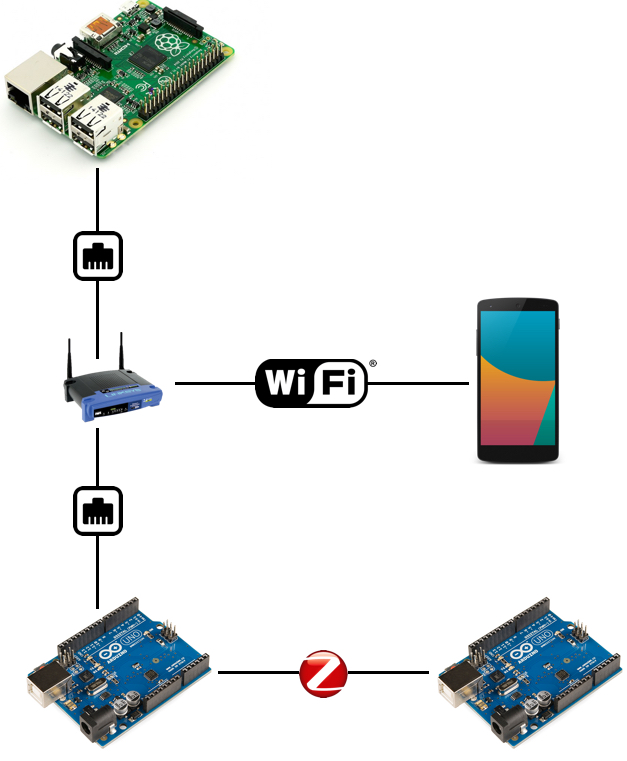
\includegraphics[width=2.5in]{Architecture}
\caption{System Architecture}
\label{fig_arch}
\end{figure}

The first subsystem is the \textit{Sensor Arduino}. This system is an Arduino that has a LDR (Light Dependent Resistor), a LED (Light Emitting Diode) and a Zig-bee module for communication. In order to provide the needed functionality, it replies to the requests defined in \textit{Appendix \ref{prot_ard}}.

The second subsystem is the \textit{Base Arduino}. This Arduino performs the role of a base station in a sensor network. It is equipped with a Zig-bee module for communication with the \textit{Sensor Arduino}. This system is responsible for issuing the requests defined in \textit{Appendix \ref{prot_ard}}. It is also equipped with an Ethernet shield, to provide communication via IP to other elements of the system, using the protocol speficied in \textit{Appendix \ref{prot_serv}}.

The third subsystem is the \textit{Server}. This system is responsible for receiving the requests to turn on or to turn off the light and to adequately reply to them. In order to to this, it implements a simple logic that specifies that the light cannot be turned on if the LDR reading is below a certain threshold. Using the protocol defined in \textit{Appendix \ref{prot_serv}}, this system communicates with the \textit{Base Arduino} to read the LDR and to operate the LED. It also provides an implementation of the protocol defined in \textit{Appendix \ref{prot_smart}}.

The final subsystem is the \textit{Android Smartphone}. This system runs an app that emulates when an user arrives to a building by sending a request to turn on the lights and when a user leaves the building by sending a request to turn off the lights, using the protocol specified in \textit{Appendix \ref{prot_smart}}.

The \textit{Base Arduino}, \textit{Server} and \textit{Android Smartphone} subsystems are connected with an IP network. The \textit{Base Arduino} is connected to the router using Ethernet, while the \textit{Android Smartphone} and the \textit{Server} use WiFi to connect to it. However, the communication between the \textit{Base Arduino} and the \textit{Sensor Arduino} is done using Zig-bee, which means that the \textit{Base Arduino} works as a relay, receiving packets from the \textit{Server} using the IP network and forwarding the requests to the \textit{Sensor Arduino} using Zig-bee.

\begin{figure*}
\centering
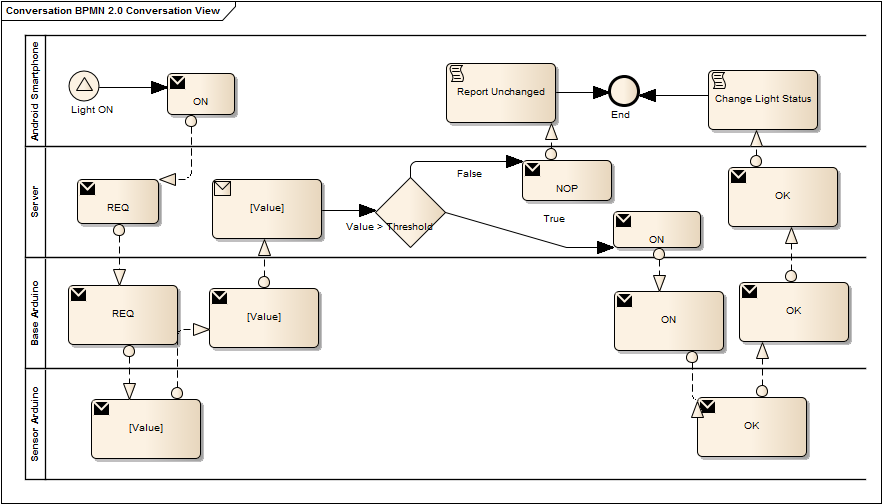
\includegraphics[width=6in]{ON_Flow}
\caption{Messages exchanged to turn on the light}
\label{fig_on_f}
\end{figure*}

\section{Network technologies used}
\label{net_tech}

To implement the described system, we used Ethernet (IEEE 802.3) and Wi-Fi (IEEE 802.11) technologies to communicate within the IP network. These technologies are mature technologies that are widely deployed for the communication scenarios used in our system.

To communicate between the Arduinos, we use ZigBee. Part of ZigBee is standardised in IEEE 802.15.4. This is a standard defined by the IEEE 802.15 working group, which is responsible for wireless personal area networks (WPAN). Another standard defined by this workgroup is Bluetooth (IEEE 802.15.1). Although ZigBee and Bluetooth are WPAN standards, their use cases differ. In table \ref{table_zb} both technologies are compared and it is shown what type of use cases they are suited for and why.

\begin{table}[h]
\centering
\begin{tabular}{lll}
Feature                              & ZigBee                                 & Bluetooth                 \\ \hline
\rowcolor[HTML]{EFEFEF} 
{\color[HTML]{333333} Channel width} & {\color[HTML]{333333} 0.3 and 0.6 MHz} & 1 MHz                     \\
Range                                & Up to 70 m                             & 10 m                      \\
\rowcolor[HTML]{EFEFEF} 
Transfer rates                       & 250 Kbps                               & 1 Mbps                    \\
Data types                           & Small data packets                     & Text, multimedia          \\
\rowcolor[HTML]{EFEFEF} 
Application types                    & Remote controls, sensors               & Mouse, Keyboard, Headsets \\
                                     &                                        &                          
\end{tabular}
\caption{Comparison of ZigBee and Bluetooth \cite{1_engineersgarage.com}}
\label{table_zb}
\end{table}

Bluetooth has a higher transfer rate which makes it more suitable for applications that require large packets to be transmitted. On the other hand, ZigBee is better suited for remote controlling objects and sensor networks, since it uses less energy and, in normal usage, batteries powering ZigBee devices can last several years. It is up to 10 times faster at switching the radio from on to off, and vice versa, than Bluetooth, making it better in use cases that require frequent exchange of small messages.

\section{Arduino setup}
\label{ard_setup}

The described sensor network was implemented with the Arduino platform. In the following sections, this report describes the components used and how they were assembled. The required components are presented in the list below.

\begin{itemize}
  \item 1 Arduino Ethernet
  \item 1 Arduino Uno
  \item 2 Arduino Wireless Proto Shield
  \item 2 Digi International XBee S1 modules
  \item 1 Tinkerkit Sensor Shield
  \item 1 Tinkerkit LED
  \item 1 Tinkerkit LDR
\end{itemize}

\subsection{Base Arduino}

The \textit{Base Arduino} was assembled with 1 Arduino Ethernet, 1 Arduino Wireless Proto Shield and 1 Digi International XBee S1 module. Figure \ref{fig_b_ard} shows the assembled \textit{Base Arduino}.

The assembled device takes advantage of the stackable shields to connect the Wireless Proto Shield to the Arduino. The XBee module is connected to the Wireless Proto Shield.

\begin{figure}[H]
\centering
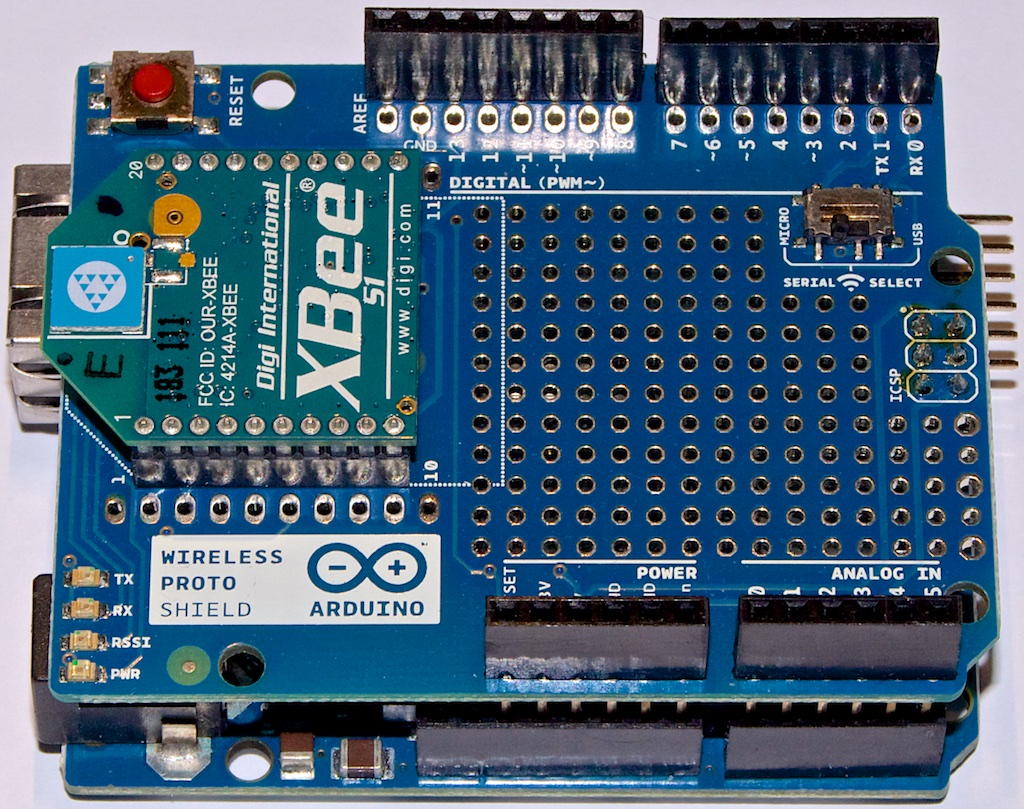
\includegraphics[width=2.5in]{Server_Arduino}
\caption{Assembled Base Arduino}
\label{fig_b_ard}
\end{figure}

\subsection{Sensor Arduino}

The \textit{Sensor Arduino} was assembled with 1 Arduino Uno, 1 Arduino Wireless Proto Shield, 1 Digi International XBee S1 module, 1 Tinkerkit Sensor Shield, 1 Tinkerkit LED and 1 Tinkerkit LDR. Figure \ref{fig_s_ard} shows the assembled \textit{Sensor Arduino} without the sensors connected to it.

As with the \textit{Base Arduino}, the \textit{Sensor Arduino} also takes advantage of the stackable shields. This Arduino is assembled the same way as the \textit{Base Arduino}, but adds the Sensor Shield on top of the Wireless Proto Shield.

The LDR and the LED are connected to the Sensor Shield using the inputs and outputs provided by it. The LDR is an input device and, as such, is connected to the inputs of the shield. To work with our code, it is connected to input 0, which maps to pin A0 in the Arduino. The LED is an output device and, as such, is connected to the outputs of the shield. To work with our code, it is connected to output 0, which maps to pin 11 in the Arduino.

\begin{figure}[H]
\centering
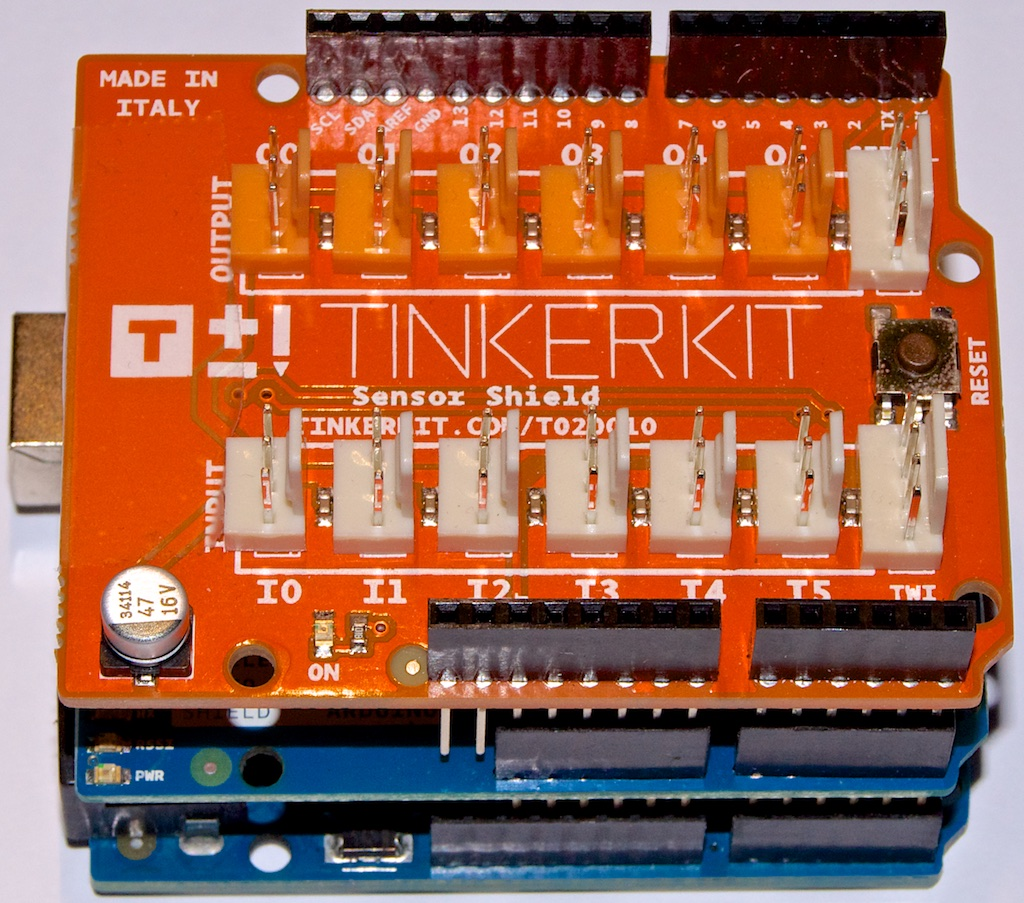
\includegraphics[width=2.5in]{Sensor_Arduino}
\caption{Assembled Sensor Arduino}
\label{fig_s_ard}
\end{figure}

\section{Communication between subsystems}
\label{comm_sub}

On our system, the \textit{Android Smartphone} acts as the controller for the simulated light bulb on the \textit{Sensor Arduino}. Yet, they are not directly connected and must, therefore, communicate using other subsystems. This is achieved by passing messages between the subsystems.

In \textit{Fig. \ref{fig_on_f}}, the messages that are exchanged when the \textit{Android Smartphone} requests to turn on the light. It also shows the logic implemented in the \textit{Server} to decide if the light should be turned on or not.

\textit{Fig. \ref{fig_off_f}} shows the message exchange for an off request issued by the \textit{Android Smartphone}. The process is simpler because there is no logic associated to this process and the \textit{Server} acts as a relay, transmitting the messages to the \textit{Base Arduino}.

\begin{figure}[H]
\centering
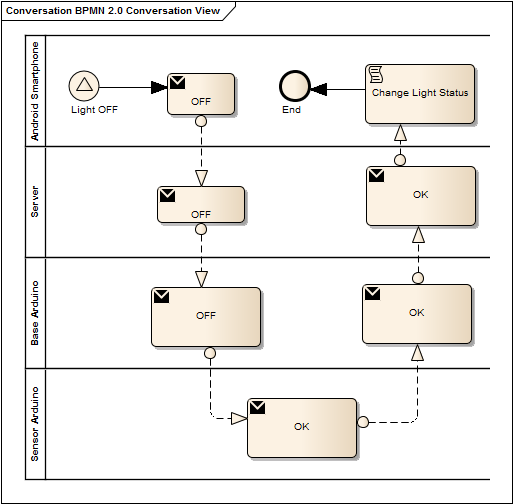
\includegraphics[width=2.5in]{OFF_Flow}
\caption{Messages exchanged to turn off the light}
\label{fig_off_f}
\end{figure}

\subsection{ZigBee network configuration}

In order to communicate with ZigBee, both the \textit{Base Arduino} and the \textit{Sensor Arduino} need to configure the XBee module with the correct parameters. In this section, the report describes the configuration performed during the setup phase of the Arduino sketches, which is based on the configuration provided in \textit{Making Things Talk} \cite[Chapter~6]{igoe2007making}.

In the experiment we needed to assign addresses for the XBee modules. This is done by issuing AT commands to the module that configure it. The commands are issued using serial communication at a rate of 9600 Bd.

The first command issued is \texttt{ATDH}, which sets the serial number of the receiving module. This value is set to \texttt{0}, which represents a broadcast, because the selection will be done by the ID in the network. The next command issued is \texttt{ATDL}, which sets the ID of the receiving module. Finally, the \texttt{ATMY} command is issued, which sets the module ID in the network. Table \ref{table_vals} shows the values used in each Arduino.

\begin{table}[h]
\centering
\begin{tabular}{lll}
Command                     & \textit{Base Arduino}    & \textit{Sensor Arduino}  \\ \hline
\rowcolor[HTML]{EFEFEF} 
{\color[HTML]{333333} ATDH} & {\color[HTML]{333333} 0} & {\color[HTML]{333333} 0} \\
ATDL                        & 1235                     & 1234                     \\
\rowcolor[HTML]{EFEFEF} 
ATMY                        & 1234                     & 1235                     \\
                            &                          &
\end{tabular}
\caption{Values of the AT commands issued}
\label{table_vals}
\end{table}

Before issuing the described commands, both Arduinos issue the command \texttt{+++} to enter the configuration mode and \texttt{ATRE} to reset the memory of the module. After issuing the described commands, the command \textit{ATWR} is issued to write the configuration to memory and \textit{ATCN} is issued to exit configuration mode.

Other AT commands are available and allow the configuration of more complex systems. One example of such commands is \texttt{ATCH}, which allows to configure the channel on which the modules communicate.

\section{System implementation}
\label{sys_impl}

To implement the described system, we have used the Arduino Language to program both Arduinos, Python to program the \textit{Server} and Java to program the \textit{Android Smartphone}. These decisions are justified in the sections below.

\subsection{Arduino Language}

The Arduino Language is similar in syntax to C, which makes it easy to learn and develop on. It supports the common control structures and operations used in other languages, even though the processing power of the Arduino is limited. Finally, it is the reference language for programming Arduinos and the language supported by the official Arduino IDE. Table \ref{table_funs} shows some of the used functions.

\begin{table}[h]
\centering
\begin{tabular}{ll}
Function                                  & Usage                                             \\ \hline
\rowcolor[HTML]{EFEFEF} 
{\color[HTML]{333333} pinMode(pin, mode)} & {\color[HTML]{333333} Used to define the LED pin} \\
digitalWrite(pin, value)                  & Used to set the value of the pin                  \\
\rowcolor[HTML]{EFEFEF} 
analogRead(pin)                           & 1234        \\
&
\end{tabular}
\caption{Used functions}
\label{table_funs}
\end{table}

Together with this functions, we used the Serial and Ethernet libraries. The Serial library provides functions to interact with the XBee modules, such as \texttt{read}, \texttt{print} or \texttt{available}. The Ethernet library provides functions to communicate in the IP network and is similar in usage to the Serial library.

Other libraries for more sophisticated tasks are available, such as connecting to a GPRS network, connecting to a Wi-Fi network or drawing text and images on a TFT screen. These libraries are not needed for our system, but demonstrate the potential of the Arduino platform and possible extensions that can be implemented into our system.

\subsection{Python}

Python was used to implement the \texttt{Server} subsystem since it allows for rapid prototyping of the implementation. Python is less verbose than C and C like languages, which facilitates reading and maintaining the code. It also provides a mature set of libraries. Since it is an interpreted language, it provides code portability, allowing the server to run on any OS and architecture that supports Python.

We use the socket library to communicate in the IP network and implement the server and the client that communicates with the \textit{Base Arduino}. The sys library is used to write a log of performed operations to a file.

The light threshold is provided when launching the \textit{Server} in the command line as an argument, thus being configurable.

\subsection{Java}

Java was chosen to implement the \textit{Android Smartphone} subsystem since it is the programming language used for Android. Android was chosen because it allows a graphical interaction with the system and provides a simulated remote control that is closer to what would be implemented in a real system.

To communicate with the \textit{Server}, we use the \texttt{Thread} class to run the communication on a different thread and the \texttt{Socket} class to communicate in the IP network. The UI is built using the libraries available in the Android SDK.

\subsection{Base Arduino}

To simplify the implementation of the \textit{Base Arduino} subsystem, we take advantage of the similarities between Appendix \ref{prot_ard} and Appendix \ref{prot_serv} protocols. Both protocols specify the same commands and replies and in the same format and their behaviour regarding errors and unknown commands is the same.

As such, our implementation of this subsystem receives a message in the IP network and relays it to the ZigBee networking, making the \textit{Sensor Arduino} responsible for correctly implementing the protocol.

\section{Extensions to the system}
\label{sys_exts}

The developed system provides a simplification of a platform that can remotely control lights and prevent the usage of the lights if there is enough light available in the room. This can be extended in multiple ways. This section presents two extensions to the system, one of which was implemented.

\subsection{Multiple lights and sensors}

The system described and implemented in this report could be extended to suit a real life scenario, where it could control a lighting system of a house. In a real life scenario, the system would have to be capable of controlling a number of different lights. The system could provide a way to adjust the light emmited in each room accordingly to the reading of the LDR, to maintain a constant light throughout the day.

A ZigBee network would be suitable for this purpose since it works well in scenarios that involve exchanging small amounts of data between the components of the network. It also has a small response time in the radio on to radio off shifting, and vice versa, and the communication can be done between a flexible number of nodes.

In this scenario, the ZigBee network could be fine tuned to allow the usage of different channels with the \texttt{ATCH} command. This would enable several nodes to transmit data simultaneously without disturbing the communication of the other nodes. This behaviour would make the system stabler and less prone to signal interference between its elements.

However, in a real life scenario, the network needs to be carefully planned to avoid interferences with Wi-Fi networks operating in the same area, since some Wi-Fi channels overlap some ZigBee channels. This can be avoided with careful planning the used channels in the Wi-Fi and ZigBee networks so that there is minimal interference between the networks.

To implement such a system, the protocols would have to be extended to support multiple lights. This could be done by associating each request with the ID of the light in the system. The \textit{Server} logic would have to be extended to support multiple lights and to keep track of them. Finally, the \textit{Android Smartphone} client would have to be redone to know in which part of the house the user is and to use the new functionalities provided by the \textit{Server}. If the system is designed to maintain a fixed amount of light in each room, the \textit{Android Smartphone} can be removed from the system since it doesn't need to be controlled.

\subsection{Guess the light! game}

The protocols designed to communicate with and within the sensor network allow its usage for different purposes than remote controlling lights. Our goal with this extension was to test its usage with a different application scenario. To do so, we have developed an extension to the Appendix \ref{prot_smart} protocol, described in Appendix \ref{prot_smart_ext}, and implemented it on the \textit{Server}.

The purpose of the \textit{Guess the light!} game is to try to guess the value that is given by the LDR, truncated to the interval [0,999]. To do so, the user must provide to a client its guess, and the client will then communicate it to the server.

When the server is launched, it requests the LDR reading to the sensor network and sets the replied value as the value to be guessed. This value can be changed at any time by the client by requesting a new reading.

When the server receives the user guest, it compares each digit with the stored value. If a digit of the guess matches a digit of the stored value, it will instruct the sensor network to blink the light once. This is done for each correct digit. Blinking the light means turning it on and then off if the light is off and turning it off and then on if the light is on.

As such, if a user correctly guesses any 2 digits of the stored value, the lights will blink twice. If a user correctly guesses the stored value, the lights will blink three times. Note that the correctly guessed digit must match the digit in the stored value. This means that if the stored value is 234 and the user guesses 342, the lights won't blink, even though the user correctly guessed all three digits, because they aren't in the right order.

\section{Conclusion}
\label{conc}

This report presents a prototype of a light control system that is capable of controlling a light and decide if that light should be turned on based on the reading of the amount of light available. It is able to correctly perform the tasks described in this report.

ZigBee has a good set of properties for developing remote control systems, specifically for the home networking systems. It provides low power consumption, low datarate and is low cost \cite{lee2013experimental}, therefore being well suited for these applications. There is also an interest by the ZigBee Aliance in further developing the standard and ZigBee products with companies with the goal to market driven requirements in the development of new features in the standard. \cite{2_the_zigbee_alliance} Setting up the ZigBee network, with the AT commands, was easy and fast. The innovative usage of the standard can further strengthen its position in the WPAN area.

We have found the syntax of the Arduino language very clear and learnable in a short amount of time, enabling developers to build ZigBee based control systems faster.

Some possible extensions to the system were discussed, including how to extend the prototype to a system capable of controlling more than one light.

\bibliographystyle{IEEEtran}
\bibliography{biblio}

\clearpage
\setcounter{page}{1}

\appendices

\section{Protocol specification for communication between arduinos}
\label{prot_ard}

The aim of this protocol is the transmission of commands from the \textit{Base Arduino} to the \textit{Sensor Arduino}. It defines the available commands as well as their replies. The commands are sent in text and have a maximum size of 3 characters. The replies are also sent in text and have a maximum size of 4 characters. Neither the commands nor the replies are terminated with any special character.

If the \textit{Sensor Arduino} receives a command that is not part of the specification, it replies with the 3 character sequence \textit{NOK}.

\subsection{REQ command}

The \textbf{REQ} command is issued for requesting the LDR's value. It is sent as the 3 character sequence \texttt{REQ}, without any special character terminating it. The expected reply to this command is a character sequence with, at most, 4 characters that represents an integer value in the range from 0 to 1023. Any other value received is an error and should be discarded.

Under normal operation, the \textit{Sensor Arduino} always executes the command.

\subsection{STS command}

The \textbf{STS} command is issued for requesting the LED's status. It is sent as the 3 character sequence \texttt{STS}, without any special character terminating it. The expected reply to this command is a character sequence with 1 character that represents an integer value. The value \texttt{0} is replied if the light is off, and \texttt{1} is replied if the light is on. Any other value received is an error and should be discarded.

Under normal operation, the \textit{Sensor Arduino} always executes the command.

\subsection{ON command}

The \textbf{ON} command is issued to turn on the LED. It is sent as the 2 character sequence \texttt{ON}, without any special character terminating it. The expected reply to this command is the character sequence \texttt{OK}, representing the successful execution of the command. Any other value received is an error and should be discarded.

Under normal operation, the \textit{Sensor Arduino} always executes the command.

\subsection{OFF command}

The \textbf{OFF} command is issued to turn off the LED. It is sent as the 3 character sequence \texttt{OFF}, without any special character terminating it. The expected reply to this command is the character sequence \texttt{OK}, representing the successful execution of the command. Any other value received is an error and should be discarded.

Under normal operation, the \textit{Sensor Arduino} always executes the command.

\section{Protocol specification for communication between server and arduino}
\label{prot_serv}

The aim of this protocol is the transmission of commands from the \textit{Server} to the \textit{Base Arduino}. It defines the available commands as well as their replies. The commands are sent in text and have a maximum size of 3 characters. The replies are also sent in text and have a maximum size of 4 characters. Neither the commands nor the replies are terminated with any special character.

If the \textit{Base Arduino} receives a command that is not part of the specification, it replies with the 3 character sequence \textit{NOK}.

\subsection{REQ command}

The \textbf{REQ} command is issued for requesting the LDR's value. It is sent as the 3 character sequence \texttt{REQ}, without any special character terminating it. The expected reply to this command is a character sequence with, at most, 4 characters that represents an integer value in the range from 0 to 1023. Any other value received is an error and should be discarded.

Under normal operation, the \textit{Base Arduino} always executes the command.

\subsection{STS command}

The \textbf{STS} command is issued for requesting the LED's status. It is sent as the 3 character sequence \texttt{STS}, without any special character terminating it. The expected reply to this command is a character sequence with 1 character that represents an integer value. The value \texttt{0} is replied if the light is off, and \texttt{1} is replied if the light is on. Any other value received is an error and should be discarded.

Under normal operation, the \textit{Base Arduino} always executes the command.

\subsection{ON command}

The \textbf{ON} command is issued to turn on the LED. It is sent as the 2 character sequence \texttt{ON}, without any special character terminating it. The expected reply to this command is the character sequence \texttt{OK}, representing the successful execution of the command. Any other value received is an error and should be discarded.

Under normal operation, the \textit{Base Arduino} always executes the command.

\subsection{OFF command}

The \textbf{OFF} command is issued to turn off the LED. It is sent as the 3 character sequence \texttt{OFF}, without any special character terminating it. The expected reply to this command is the character sequence \texttt{OK}, representing the successful execution of the command. Any other value received is an error and should be discarded.

Under normal operation, the \textit{Base Arduino} always executes the command.

\section{Protocol specification for communication between smartphone and server}
\label{prot_smart}

The aim of this protocol is the transmission of commands from the \textit{Android Smartphone} to the \textit{Server}. It defines the available commands as well as their replies. The commands are sent in text and have a maximum size of 4 characters. The replies are also sent in text and have a maximum size of 4 characters. The commands and the replies are terminated with the special character \texttt{\textbackslash n}.

If the \textit{Server} receives a command that is not part of the specification, it replies with the 4 character sequence \textit{NOK\textbackslash n}.

\subsection{ON command}

The \textbf{ON} command is issued to turn on the LED. It is sent as the 3 character sequence \texttt{ON\textbackslash n}. The expected reply to this command is the character sequence \texttt{OK\textbackslash n}, representing the successful execution of the command.

Under normal operation, the \textit{Server} may not execute the command. This is signaled by replying with the character sequence \texttt{NOP\textbackslash n}. Any other value received is an error and should be discarded.

\subsection{OFF command}

The \textbf{OFF} command is issued to turn off the LED. It is sent as the 4 character sequence \texttt{OFF\textbackslash n}. The expected reply to this command is the character sequence \texttt{OK\textbackslash n}, representing the successful execution of the command. Any other value received is an error and should be discarded.

Under normal operation, the \textit{Server} always executes the command.

\subsection{STS command}

The \textbf{STS} command is issued for requesting the LED's status. It is sent as the 4 character sequence \texttt{STS\textbackslash n}. The expected reply to this command is a character sequence with 2 characters that represents an integer value. The value \texttt{0\textbackslash n} is replied if the light is off, and \texttt{1\textbackslash n} is replied if the light is on. Any other value received is an error and should be discarded.

Under normal operation, the \textit{Server} always executes the command.

\vfill\eject

\section{Game extensions to the Appendix \ref{prot_smart} protocol}
\label{prot_smart_ext}

The aim of this extension to the protocol described in \textit{Appendix \ref{prot_smart}} is the transmission of commands from the \textit{Client} to the \textit{Server} to control the game. The commands are sent in text and have a maximum size of 8 characters. The replies are also sent in text and have a maximum size of 4 characters. The commands and replies are terminated with the special character \texttt{\textbackslash n}.

If the \textit{Server} receives a command that is not part of the specification, it replies with the 4 character sequence \textit{NOK\textbackslash n}.

\subsection{RES command}
The \textbf{RES} command is issued to reset the value that the user has to guess. It is sent as the 4 character sequence \texttt{RES\textbackslash n}. The expected reply to this command is the character sequence \texttt{OK\textbackslash n}, representing the successful execution of the command. Any other value received is an error and should be discarded.

Under normal operation, the \textit{Server} always executes the command.

\subsection{G command}
The \textbf{G} command is issued to send the user's guess. It is sent as the 8 character sequence \texttt{G X Y Z\textbackslash n}, where \texttt{X} represents the most significant digit of the guess, \texttt{Y} the second most significant digit of the guess, and \texttt{Z} the least significant digit of the guess. The expected reply to this command is the character sequence \texttt{OK\textbackslash n}, representing the successful execution of the command. Any other value received is an error and should be discarded.

Under normal operation, the \textit{Server} always executes the command.

\end{document}